\documentclass[]{spie}  %>>> use for US letter paper
%\documentclass[a4paper]{spie}  %>>> use this instead for A4 paper
%\documentclass[nocompress]{spie}  %>>> to avoid compression of citations

\renewcommand{\baselinestretch}{1.0} % Change to 1.65 for double spacing
 
\usepackage{amsmath,amsfonts,amssymb}
\usepackage{graphicx}
\usepackage[colorlinks=true, allcolors=blue]{hyperref}
\usepackage{textcomp}
\usepackage[T1]{fontenc}
\usepackage[utf8]{inputenc}
\inputencoding{utf8}

\title{Development and validation of the Overlap Muon Track Finder for the CMS experiment}

\author[a]{J. Dobosz}
\author[a,b]{P. Miętki}
\author[a]{K. Zawistowski}
\author[a]{G. Żarnecki}
\affil[a]{University of Warsaw, Faculty of Physics, Pasteura~5, 02-093 Warsaw, Poland}
\affil[b]{Gdansk University of Technology, Faculty of Applied Physics and Mathematics,  Narutowicza~11/12, 80-233 Gdansk, Poland}

% Option to view page numbers
\pagestyle{empty} % change to \pagestyle{plain} for page numbers   
%\setcounter{page}{301} % Set start page numbering at e.g. 301

 
\begin{document} 
\maketitle

\begin{abstract}

Present article is a description of the authors contribution in upgrade and analysis of performance of the Level-1 Muon Trigger of the CMS experiment. The authors are students of University of Warsaw and Gdansk University of Technology. They are collaborating with the CMS Warsaw Group. This article summarise student's work presented during the Students session during the Workshop XXXVIII-th IEEE-SPIE Joint Symposium Wilga 2016.

In the first section the CMS experiment is briefly described and the importance of the trigger system is explained. There is also shown basic difference between old muon trigger strategy and the upgraded one.

The second section is devoted to Overlap Muon Track Finder (OMTF). This is one of the crucial components of the Level-1 Muon Trigger. The algorithm of OMTF is described.

In the third section there is discussed one of the event selection aspects - cut on the muon transverse momentum $p_{T}$. Sometimes physical muon with $p_{T}$ bigger than a certain threshold is unnecessarily cut and physical muon with lower $p_{T}$ survives. To improve $p_{T}$ selection modified algorithm was proposed and its performance was studied.

One of the features of the OMTF is that one physical muon often results in several muon candidates. The Ghost-Buster algorithm is designed to eliminate surplus candidates. In the fourth section this algorithm and its performance on different data samples are discussed.

In the fifth section Local Data Acquisition System (Local DAQ) is briefly described. It supports initial system commissioning. The test done with OMTF Local DAQ are described.  

In the sixth section there is described development of web application used for the control and monitoring of CMS electronics. The application provides access to graphical user interface for manual control and the connection to the CMS hierarchical Run Control.
\end{abstract}


% Include a list of keywords after the abstract 
\keywords{Muon Trigger, OMTF}

\section{COMPACT MUON SOLENOID AND EVENT SELECTION}
\label{sec:1_CMS}

The Compact Muon Solenoid(CMS) experiment is a general purpose particle detector in Large Hadron Collider (LHC) at European Organization for Nuclear Research (CERN).
In the first phase of research in CMS there was discovered the Higgs boson in 2012 (as well as in ATLAS experiment).
It is necessary to select events because of very high rate of proton-proton collisions and limited ability of saving produced data.
This preliminary selection of events for futher analysis is made by system called the muon trigger system.
For good operating, trigger should be as effective as it is possible with purity kept in a high level.
This mean, it should accept all intresting muons and reject the rest.
After the first operational LHC run, all of the trigger system are modernized because of increase of the luminosity and the collison energy in LHC.
The CMS Warsaw Group is working on Level-1 Muon Trigger for CMS.
In the current modernisation phase we are creating a new trigger for the overlap range, that is the area that muons cross detectors in both barrel and endcap parts.




\section{THE MUON SELECTION IN THE DETECTOR OVERLAP REGION}

The algorithm fo the Overlap Muon Track Finder (OMTF) was designed to reconstruct muon tracks in the Overlap region at the Level-1 Muon Trigger. The algorithm is based on comparing measured hits with precomputed track patterns, so-called Golden Patterns (GPs). Each GP corresponds to the muon track with a certain charge (i.e. $\mu^{+}$, $\mu^{-}$) and transverse momentum. GP comprises information about track's average azimuthal angle bending $\Delta \phi_{mean}$ between reference layer and every other layer caused by CMS magnetic field. There are also included Probability Density Function (PDF) values of possible deviations from $\Delta \phi_{mean}$ values (due to stochastic effects: multiple scattering and energy losses). 

Constant set of 8 reference layers is foreordained. In the beginning of the algorithm, up to 4 reference hits in reference layers are chosen (among all physical hits in the event) to make possible finding multiple muon candidates. Then for every signal from the event there is calculated the azimuthal angle difference $\Delta \phi_{i}$ between certain reference hit and each hit laying in acceptable logic region. In order to compare this with certain Golden Pattern algorithm calculates difference between average azimuthal angle track bending for given GP and actual track bending ($\phi_{dist} = \Delta\phi_{mean} - \Delta\phi_{i}$)% (Fig. \ref{algorithm})
 for every hit. For each layer hit with the smallest $\phi_{dist}$ value is chosen and corresponding PDF value is taken. If the PDF value is bigger than 0, the processed layer is counted as an \textit{active layer}. Subsequently the PDF values from all layers are added up. In the end for each reference hit there is chosen one Golden Pattern fitted best to event hits. The basic criterion for that choice is the number of \textit{active layers} corresponding to each GP - the pattern with more \textit{active layers} is favoured. If that number is the same for a few GPs then the pattern with the biggest sum of PDF values is selected. As this procedure is followed for up to 4 reference hits, on the output there are up to 4 candidates in the Overlap region per one event.

Described algorithm was developed on the grounds of Monte Carlo simulations and is implemented in dedicated electronics as a FPGA firmware.
%
\cite{OMTF-Wilga2014}


\section{OPTIMISATION OF EVENT SELECTION}  

In the CMS experiment there are many proton-proton beams collisions which produce lots of detected events data.
Since there is a huge rate (40MHz) of bunch crossings, it is impossible to save and analyse all of the data.
The event selection is an essential stage in the OMTF and it is being done by a trigger.
The reduction of rate is achieved by rejecting these events that are unattractive in experiment.
So the trigger has to reconstruct muon tracks in each event to make a so-called cut.
The cut consists in rejecting muons with transverse momentum lower than a specified threshold value and accept that events with a bigger one.

In the Fig. \ref{eff} there is a plot of efficiency of trigger for a momentum cut set on 16 GeV/c vs transverse momentum of muons.
The efficiency is defined as a ratio of number of accepted muons to number of all muons.
The ideal efficiency curve should look like a step function changing the efficiency value from 0 to 1 in the threshold value point.

There were performed tests of optimisation of event selection.
In this study were used data samples with simulated single muon events
The current event selection algorithm is based on quality and PDF value.
The improved one takes into consideration diversity of efficiency of each reference layer and adds different relevance to PDF sub-values that depends on detector type.
The RPC detectors was devalued because of their poor spatial resolution, the weight for DT detectors was increased due to their excellent spatial resolution.
For CSC detectors there were no changes.
In the Fig. \ref{eff} there is plot of these two options of muon selection in OMTF - actual and improved.
They are compared with the best possible efficiency for that case that is known because it is plotted on simulated Monte Carlo data. %not redundant information IMHO, no comma before "that".

\begin{figure}[ht]
\centering
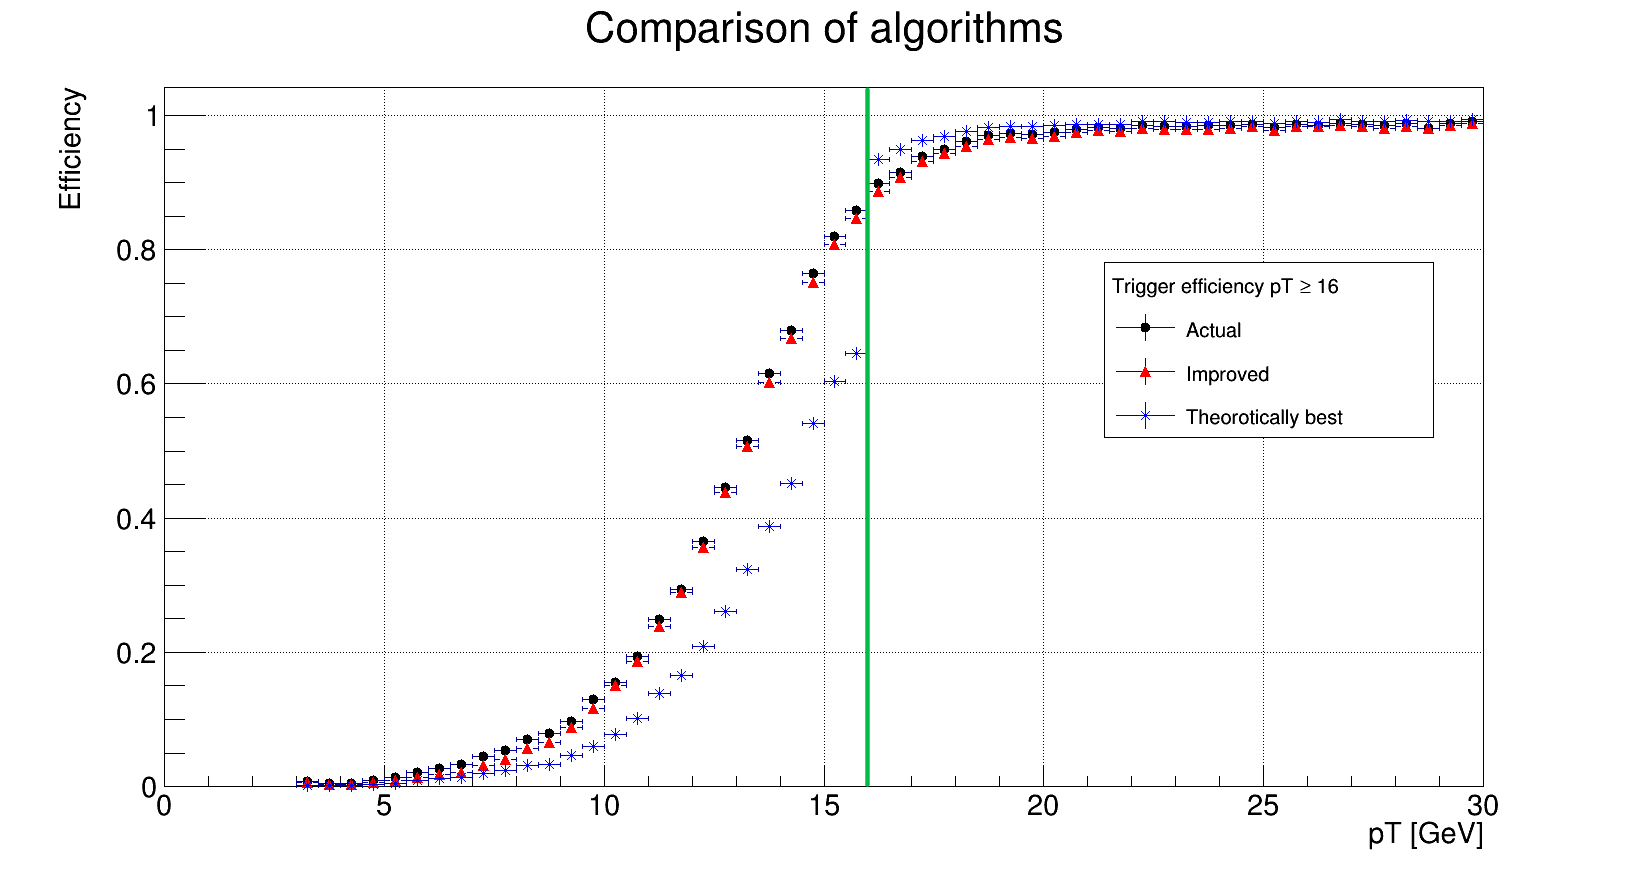
\includegraphics[width=0.9\textwidth]{Hist16.png}
\caption{Efficiency of different algorithms of events selection vs muon transverse momentum}
\label{eff}
\end{figure} 

The selection in the range below the momentum cut is essential because it improves the purity of the trigger.
It is important since low-energetic muons increase a difficulty of data analysis.
In the Fig. \ref{ratio} there is a plot of ratio of previous efficiencies that shows some improvement in range of low transverse momentum.

\begin{figure}[ht]
\centering
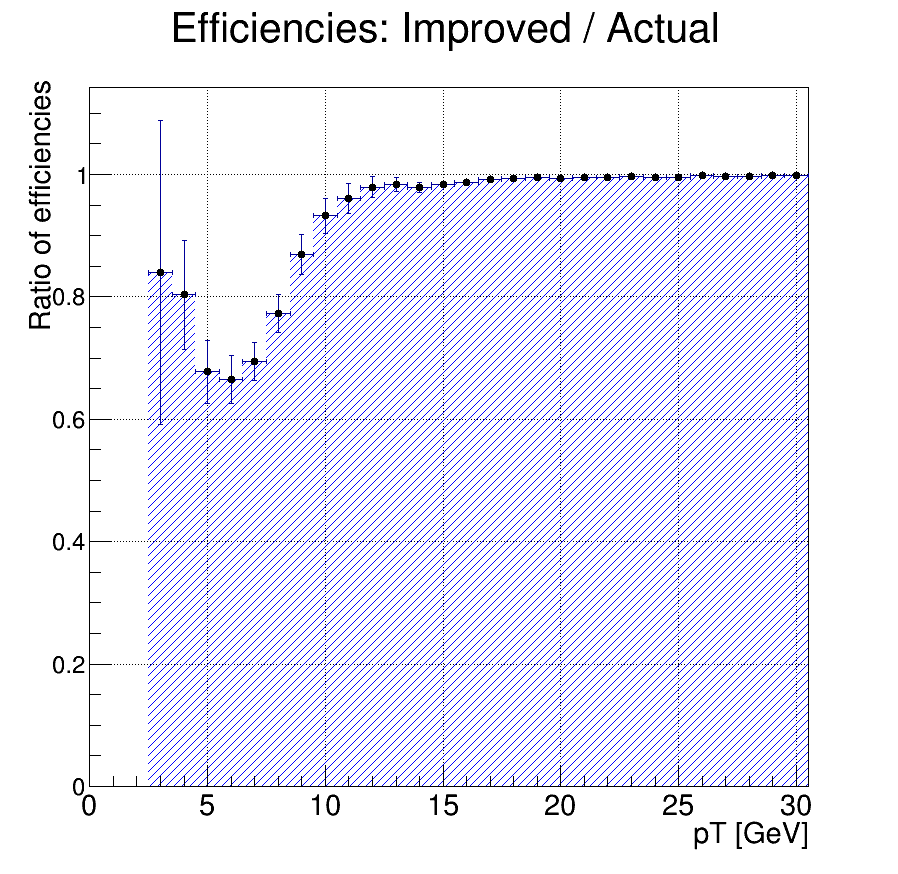
\includegraphics[width=0.5\textwidth]{Ratio16.png}
\caption{Ratio of improved efficiency and actual efficiency. Muons with momentum in the range from 3 to 12 GeV are rejected in a better way.}
\label{ratio}
\end{figure} 



\section{TEST OF GHOST BUSTER ALGORITHM}

During the step of muon track reconstruction it is common that one physical muon causes a few muon candidates with similar track parameters. The additional candidates are often called \textit{ghosts}. The step of eliminating \textit{ghosts} is called GhostBuster. GhostBuster takes the input set of muon candidates and produces the output set of selected candidates. The algorithm of GhostBuster is based on comparing azimuthal angle of muon candidates. Sometimes two or more physical muons appear in Overlap region per one event. Well working GhostBuster is expected to select the same number of muon candidates as the number of physical muons. For the present article performance of GhostBuster emulator was studied.

In the beginning the input set of candidates is taken and they are sorted by quality. Then all candidates are checked in a loop whether their azimuthal angle is close to the azimuthal angle of candidates which are already in the output set (that is performed in a nested loop). If the angle difference is smaller than veto \textit{window} (set to 5\textdegree) then the candidate from the input set is recognized as a \textit{ghost} and is not passed to the output set. Consequently input candidate with the best quality is always forwarded to the output set.

Chance for finding and eliminating \textit{ghosts} successfully depends significantly on the width of the veto \textit{window}. To study this dependancy data samples with simulated single muon events were used. In the Fig. \ref{prob_vs_phi} there is a plot of probability of getting certain number of candidates at the GhostBuster output set vs veto \textit{window} width. This plot was done for events with both generated muons propagating into the whole Overlap region, that is with pseudorapidity $0.83 < \eta < 1.24$.
\begin{figure}[ht]
\centering
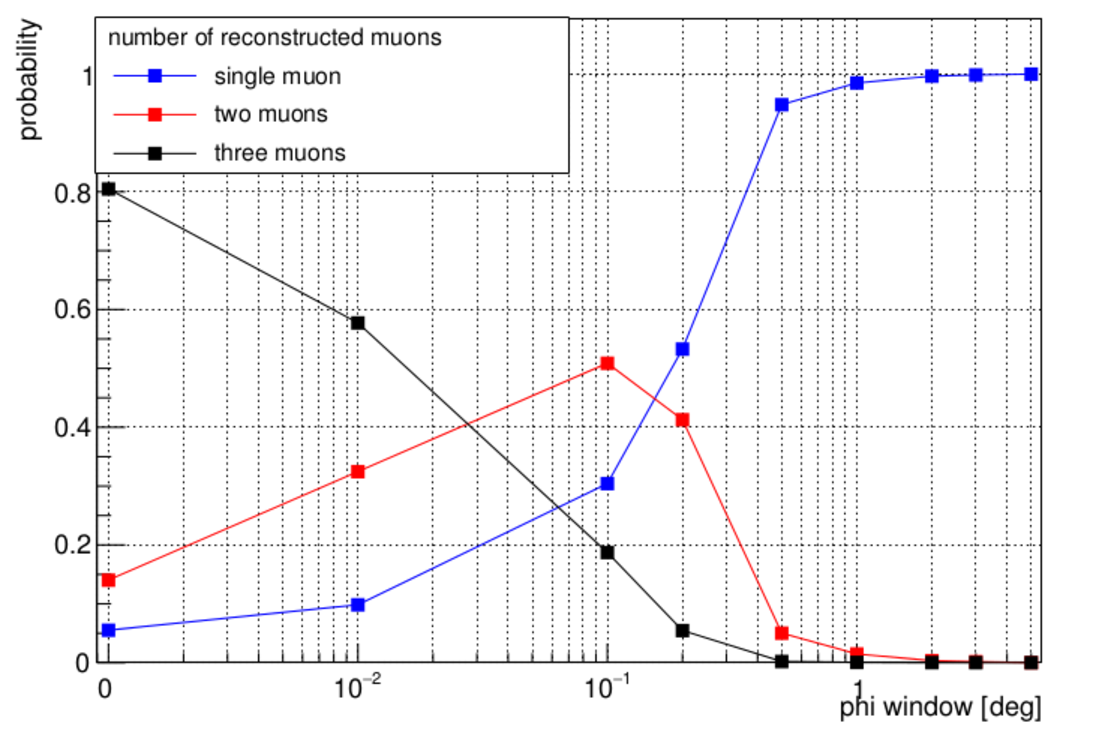
\includegraphics[width=0.7\textwidth]{prob_phi.pdf}
\caption{Results obtained for sample with single muon events. Probability of multiple muon reconstruction on the output of GhostBuster vs $\phi$ \textit{window} width. Points on the left edge of plot refer to \textit{window} width set to 0\textdegree. }
\label{prob_vs_phi}
\end{figure} 
For the very small values of veto \textit{window} width GhostBuster's performance is degenerated - in most cases single physical muon will be reconstructed as multiple candidates. For 0.5\textdegree\textrm{ }and 1\textdegree\textrm{ }GhostBuster is clearly much more effective and for 5\textdegree\textrm{ }probability of receiving single candidate on the output set is bigger than 99.9\%. 

Good \textit{ghosts} selection has however its price. For high transverse momenta GhostBuster decreases efficiency of the $\mu^{+}\mu^{-}$ pairs reconstruction. This effect was studied on data samples with simulated single J/$\Psi \rightarrow \mu^{+}\mu^{-}$ decay events. In the Fig. \ref{divmom} there is a plot of efficiency of the $\mu^{+}\mu^{-}$ pairs reconstruction vs J/$\psi$ generated transverse momentum. This plot was done for events with both generated muons propagating into the middle Overlap region, that is with pseudorapidity $0.9 < \eta < 1.15$. For J/$\psi$ transverse momentum bigger than 40 GeV/c efficiency drops from $(92.4\pm0.5)\%$ (when cut on azimuthal angle is disabled) to $(86.2\pm0.6)\%$ (when 5\textdegree cut is used). This is a consequence of fact that for high J/$\psi$ momenta the decay resulting in muons propagating into narrow $\phi$ \textit{window} is more probable.
\begin{figure}[ht]
\centering
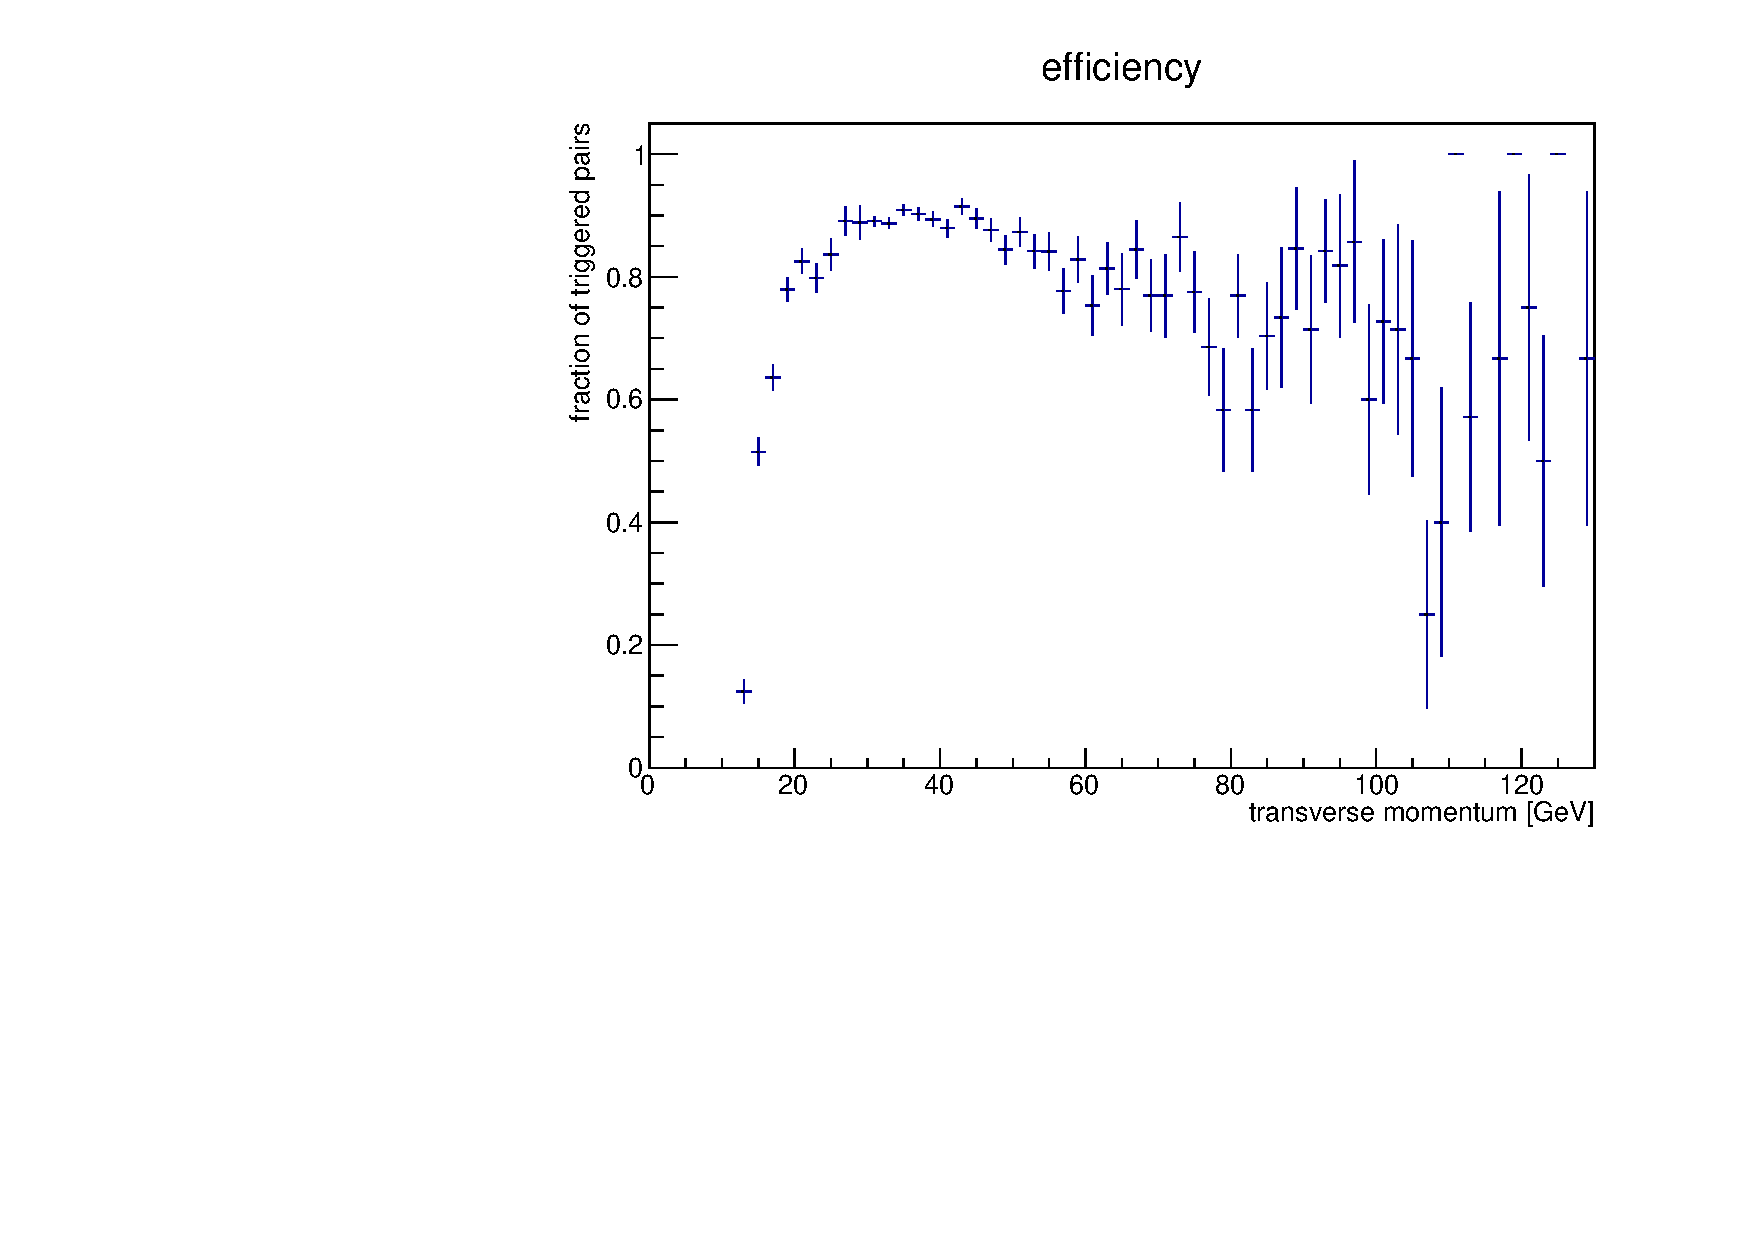
\includegraphics[width=0.7\textwidth]{efficiency_GB_5.pdf}
\caption{Efficiency of reconstructing two muon candidates vs J/$\psi$ transverse momentum.}
\label{divmom}
\end{figure} 


\section{SYSTEM TESTS WITH LOCAL DATA}
For further reconstruction analysis CMS was equipped with Data Acquisition
System (DAQ), which saves cases selected by detector. Regardless of
it, OMTF introduced ability to read data directly from memory buffers.
This readout set was called Local Data Acquisition System (Local DAQ)
and it is a kind of \textit{spy module}, which means it allows to snapshot
some raw data collected by detectors for further hits correlation
or system feedback analysis.

Local DAQ returns 3 steps of data acquisition and analysis - raw hits
collected by detectors (AlgoHits), data after selection by hardware-built-in
algorithm (AlgoMuons) and data after ghostbusting (CandMuons). There
is too much data being processed by hardware at one point of time,
so Local DAQ reads it with bounded bandwith.

Data collected from Local DAQ can be analysed to check angular distribution
of hits in the barrel region. It is expected to be uniform with some
fluctuations in the chamber overlapping region. If expectations are
met, it means that detectors work properly and give CMS statistically
correct data.

Other important things to check are correlations of hits between chambers.
Due to geometry of OMTF, some chambers are placed directly next to
others (RPC and DT in barrel region or RPC and CSC in endcap region).
This allows to check whether detectors work properly by data correlation
analysis. If AlgoMuons data is included, hardware algorithm work may
be checked either.

The next step in local data analysis is to compare results of hardware-built-in
algorithm with outcome of emulation of algorithm work. There are plenty
of features to check such as muon energy, muon momentum, hit phi angle
and so on. Such analysis will help to upgrade algorithm and in effect
total efficiency of OMTF.


\section{SYSTEM CONTROL AND MONITORING} 
A dedicated web application is used for the monitoring and control of CMS electronics. As the new Level-1 Trigger uses standardised electronics designs and standard communication protocol, significant effort has been made to provide shared implementation of low level functionalities that are common across different Level-1 subsystems.
This gave rise to SWATCH, a specialised web container for upgraded Level-1 Trigger control application, and MicroHAL, a high-level hardware control library. The structure of the OMTF Control Software is defined by the usage of these components, as it
comprises two basic modules: OMTF System, a SWATCH-based web application, and OMTF Hardware Control.

OMTF System was built upon SWATCH-based abstractions of the system, the state of the system, operations executed on the hardware, and large scale hardware components. It provides access to many features granted by SWATCH framework, such as 
graphical user interface for diagnostics, monitoring and manual control, the connection to the CMS hierarchical Run Control allowing the subsystem to be operated automatically with the rest of Level-1 trigger and standardised configuration using relational 
database provided by ORACLE.

OMTF Hardware Control contains implementations of various hardware routines required to operate the system. It makes use of detailed tree-like firmware description provided by MicroHAL library and wraps it in it's own object oriented description, to provide
compile-time validation, integration with the code analysis engine provided by the integrated development environment and additional order and convenience. The object reflection is split into two parts: blueprint base classes, generated automatically 
from the firmware description used by MicroHAL, and the subclasses containing needed implementations.

Both aforementioned components are written in C++ and compiled to dynamical shared libraries with use of the standardised Make scripts used normally by the majority of CMS online processing software.

As the OMTF hardware makes use of firmware blocks and hardware designs developed for other Level-1 subsystems, the components of supplied software were integrated into OMTF software when possible. 



\acknowledgments % equivalent to \section*{ACKNOWLEDGMENTS}       
 
Work supported by National Science Centre, Poland, grant 2013/11/B/ST2/04202. 

% References
\bibliography{biblio} % bibliography data in report.bib
\bibliographystyle{spiebib} % makes bibtex use spiebib.bst

\end{document} 
